\documentclass{article}

\usepackage[letterpaper, portrait, margin=1.5in]{geometry}

\usepackage{fancyhdr}
\usepackage{ragged2e}
\usepackage{graphicx}
\usepackage{caption}
\usepackage{amsmath}
\usepackage{rotating}

\usepackage{listings}
\usepackage{color}

\definecolor{dkgreen}{rgb}{0,0.6,0}
\definecolor{gray}{rgb}{0.5,0.5,0.5}
\definecolor{mauve}{rgb}{0.58,0,0.82}

\lstset{frame=tb,
  language=Java,
  aboveskip=3mm,
  belowskip=3mm,
  showstringspaces=false,
  columns=flexible,
  basicstyle={\small\ttfamily},
  numbers=none,
  numberstyle=\tiny\color{gray},
  keywordstyle=\color{blue},
  commentstyle=\color{dkgreen},
  stringstyle=\color{mauve},
  breaklines=true,
  breakatwhitespace=true,
  tabsize=4
}

\setcounter{secnumdepth}{1}

\usepackage{chngcntr}
\counterwithin{figure}{section}

\renewcommand*{\thepage}{C\arabic{page}}

\pagestyle{fancy}
\lhead{ACME Robotics}
\chead{\#8367}
\rhead{\ifcontents Contents \else Week \thesection \fi}

\newif\ifcontents
\contentstrue

\makeatletter
\renewcommand{\@seccntformat}[1]{}
\makeatother
\begin{document}

\subsection{Intake Gate}
%! Creating a servo powered gate at the back of the intake.
After completing the attachment of the diverter to the robot the entire intake was almost complete. Aidan realized that to meet the two materials maximum rule the intake was going to need another gate that would stop any more materials from going into the diverter. Previously the team had thought that this problem was already taken care of with the cartridge itself. The cartridge was supposed to be able to only hold two and then the gate at the top of the cartridge would close and stop any excess minerals. This was not going to work because the way that gate closed would actually pull in more minerals and get them caught in the robot. To fix this problem a gate needed to be created at the top of the intake. Shawn created this gate as shown in figure \ref{fig:gate} . This fixed the problem because it stopped any extra minerals from going into the diverter and the extra minerals could easily be repelled with the intake running reverse.

\begin{figure}
    \centering
    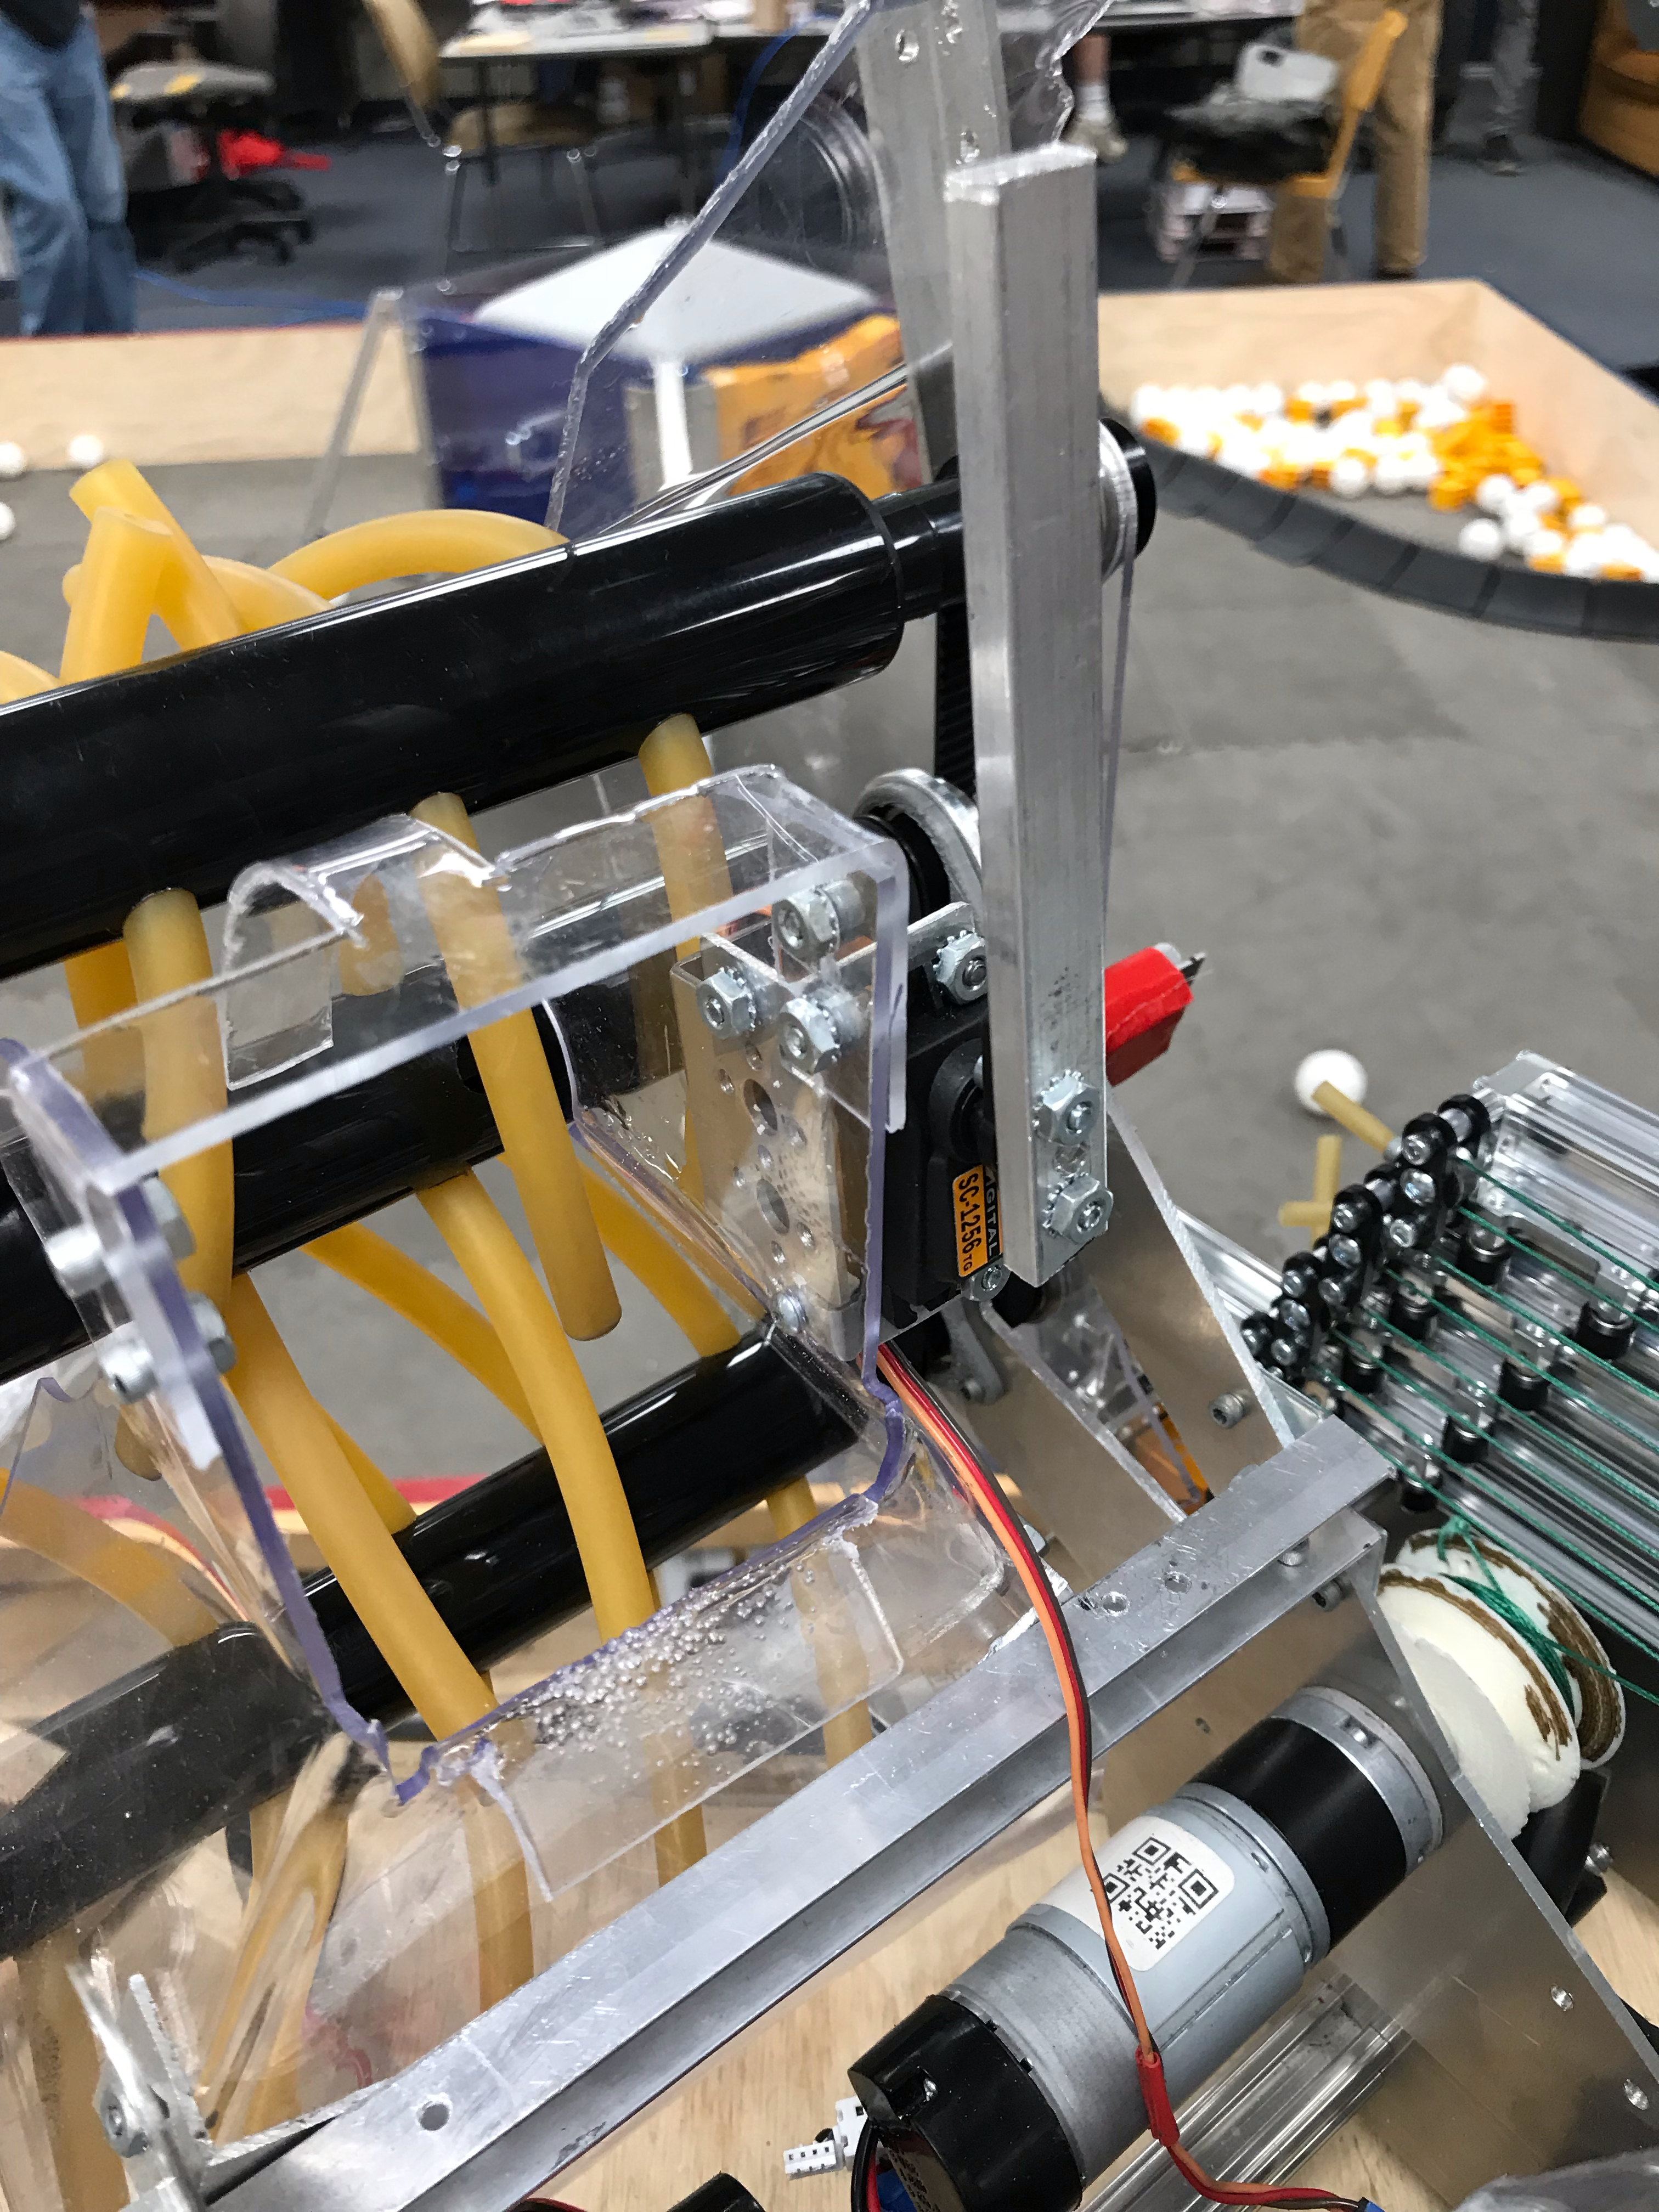
\includegraphics[height=6cm]{16_12-17/images/gate.jpg}
    \caption{Intake Gate}
    \label{fig:gate}
\end{figure}

\subsection{Attaching the rake and testing the intake}
%! Finding and testing a different way to attach the X-rail
Now that all systems of the intake at least had a  prototype, the team wanted to attach them all to the robot for testing. The team quickly ran into complications with the rake however. Originally, ACME planned to mount the rake in a similar fashion the the Rev linear slides by bolting the bottom to the outside drive plate. However, the X-rail was much taller and longer then the Rev slides; meaning the servo the rake mounted to would be to high off the ground and outside the 18'. The team first tried to mount the servo lower with a long bracket. This turned out to be too flimsy and was quickly scrapped. Next the team tried an elongated arm from the servo to the rake. This produced similar problems of stability and got in the way of deployment. The team then discovered that they could mount the X-rail upside down by mounting it from outside drive plate. This solved the issue of the servo being too high up and far out. It would also streamline the whole design and was stronger than any previous solutions. After some brainstorming about how exactly to mount it the team decided on cutting a new outside drive plate with an extended top that would curve over and mount to the top of the X-rail via bolts. (Fig 0.2). To test this idea, the team created a prototype and mounted it to the robot. This way they could test if it was feasible before cutting a new drive plate. Which would use valuable material and time. The tests were successful and the team is going ahead with the design. 

\begin{figure}
    \centering
    \includegraphics[height=6cm]{16_12-17/images/x-rail_mount.JPG}
    \caption{Sketch of X-rail mount on the outside drive plate}
    \label{fig:Mount Sketch}
\end{figure}

\begin{figure}
    \centering
    \includegraphics[height=6cmangle=90,origin=c]{16_12-17/images/mount_proto.JPG}
    \caption{Prototype outside drive plate mount}
    \label{Prototype Mount}
\end{figure}

\subsection{Building the pulley system for the lift}
%!This week, Ben made the pulley system for the lift.

This week Ben worked on developing the pulley system for the lift. He started thinking that he might use pulleys and tetrix L Brackets that already had holes so that he didn't have to cut new ones. Ben then cut down the side on on of them to try to get the bracket as close as possible to the side of the lift. He then used some v bearings to be able to string it. Then, after he adjusted the design, he made two more to put at the bottom and one to go at the top.

\subsection{Deconstructing Robot}
After all the sub-systems had been tested Oren,Ben,Shawn, and Adian took apart the main portion of the robot, as to prepare for the coming week. They made sure to organize and keep all the necessary parts to make a smooth re-construction of version 2.0. There was a considerable amount of modifications made to fully built subsystems to make sure they would fit on the new drive-train. One of the changes that had to be made was to the intakes rollers length, due to the inner dimension of the aluminum plates increasing, which in turn increased the length of the rollers. 
\end{document} 

 